\documentclass[12pt]{article}
%\usepackage[english]{babel}
\usepackage{graphicx}
%\usepackage{framed}
%\usepackage[normalem]{ulem}
\usepackage{indentfirst}
\usepackage{amsmath,amsthm,amssymb,amsfonts}
\numberwithin{equation}{section}
\usepackage{mathtools}
\usepackage[italicdiff]{physics}
\usepackage[T1]{fontenc}
\usepackage{lmodern,mathrsfs}%font
\usepackage[inline,shortlabels]{enumitem}
\setlist{topsep=2pt,itemsep=2pt,parsep=0pt,partopsep=0pt}
\usepackage[dvipsnames]{xcolor}
\usepackage[utf8]{inputenc}
%\usepackage[letterpaper, top=0.5in,bottom=0.2in, left=0.5in, right=0.5in, footskip=0.3in, includefoot]{geometry}
\usepackage[letterpaper,left=0.5in, right=0.5in,top=0.7in,bottom=1in,footskip=0.3in,includefoot]{geometry}

\usepackage[most]{tcolorbox}
\usepackage{tikz,tikz-3dplot,tikz-cd,tkz-tab,tkz-euclide,pgf,pgfplots,tikz-feynman}
\pgfplotsset{compat=newest}


\usepackage{multicol}
\usepackage[bottom,multiple]{footmisc} 
%\usepackage[backend=bibtex,style=numeric]{biblatex}
%\addbibresource{bibliography}
\usepackage{hyperref}
\hypersetup{
    colorlinks=true,
    linkcolor=magenta,
    filecolor=pink,      
    urlcolor=cyan,
    pdftitle={QFTCS Note},
    pdfpagemode=FullScreen,
    }
\usepackage[titletoc, toc, page]{appendix}
\usepackage{subfiles}



\newtheoremstyle{1style}{}{}{}{}{\sffamily\bfseries}{.\\}{ }{}
\newtheoremstyle{2style}{}{}{}{}{\sffamily\bfseries}{\\}{ }{}
%\newtheoremstyle{cstyle}{}{}{}{}{\sffamily\bfseries}{}{ }{\thmnote{#3}}

\theoremstyle{1style}
\newtheorem{definition}[equation]{Definition}
\newtheorem{theorem}[equation]{Theorem}
\newtheorem{example}[equation]{Example}
\newtheorem{cthm}[equation]{}
\newtheorem*{remark}{Remark}


%\theoremstyle{mystyle}{\newtheorem{proposition}[definition]{Proposition}}
%\theoremstyle{mystyle}{\newtheorem{lemma}[definition]{Lemma}}
%\theoremstyle{mystyle}{\newtheorem{corollary}[definition]{Corollary}}
%\theoremstyle{mystyle}{\newtheorem*{remarks}{Remarks}}
%\newtheorem{examples}{Examples}[equation]
%\theoremstyle{definition}{\newtheorem*{exercise}{Exercise}}



\tcolorboxenvironment{definition}
{boxrule=0pt,boxsep=0pt,colback={red!10},left=8pt,right=8pt,enhanced jigsaw, borderline west={2pt}{0pt}{red},
sharp corners,before skip=10pt,after skip=10pt,breakable}
\tcolorboxenvironment{theorem}
{boxrule=0pt,boxsep=0pt,colback={MidnightBlue!10},left=8pt,right=8pt,enhanced jigsaw, borderline west={2pt}{0pt}{MidnightBlue},
sharp corners,before skip=10pt,after skip=10pt,breakable}
\tcolorboxenvironment{example}
{boxrule=0pt,boxsep=0pt,colback={Magenta!10},left=8pt,right=8pt,enhanced jigsaw, borderline west={2pt}{0pt}{Magenta},
sharp corners,before skip=10pt,after skip=10pt,breakable}
\tcolorboxenvironment{proof}
{boxrule=0pt,boxsep=0pt,blanker,borderline west={2pt}{0pt}{CadetBlue!80!white},left=8pt,right=8pt,
sharp corners,before skip=10pt,after skip=10pt,breakable}
\tcolorboxenvironment{cthm}
{boxrule=0pt,boxsep=0pt,colback={orange!10},left=8pt,right=8pt,enhanced jigsaw, borderline west={2pt}{0pt}{orange},
sharp corners,before skip=10pt,after skip=10pt,breakable}
\tcolorboxenvironment{equation}
{boxrule=0pt,boxsep=0pt,colback={Green!10},left=8pt,right=8pt,enhanced jigsaw, borderline west={2pt}{0pt}{Green},
sharp corners,before skip=10pt,after skip=10pt,breakable}
\tcolorboxenvironment{align}
{boxrule=0pt,boxsep=0pt,colback={blue!10},left=8pt,right=8pt,enhanced jigsaw, borderline west={2pt}{0pt}{blue},
sharp corners,before skip=10pt,after skip=10pt,breakable}
\tcolorboxenvironment{remark}
{boxrule=0pt,boxsep=0pt,blanker,borderline west={2pt}{0pt}{Cyan},left=8pt,right=8pt,before skip=10pt,after skip=10pt,breakable}

%\tcolorboxenvironment{proposition}{boxrule=0pt,boxsep=0pt,colback={Orange!10},left=8pt,right=8pt,enhanced jigsaw, borderline west={2pt}{0pt}{Orange},sharp corners,before skip=10pt,after skip=10pt,breakable}
%\tcolorboxenvironment{examples}{boxrule=0pt,boxsep=0pt,colback={violet!10},left=8pt,right=8pt,enhanced jigsaw, borderline west={2pt}{0pt}{violet},sharp corners,before skip=10pt,after skip=10pt,breakable}
%\tcolorboxenvironment{remarks}{boxrule=0pt,boxsep=0pt,blanker,borderline west={2pt}{0pt}{Green},left=8pt,right=8pt,before skip=10pt,after skip=10pt,breakable}
%\tcolorboxenvironment{example}{boxrule=0pt,boxsep=0pt,blanker,borderline west={2pt}{0pt}{Black},left=8pt,right=8pt,sharp corners,before skip=10pt,after skip=10pt,breakable}
%\tcolorboxenvironment{examples}{boxrule=0pt,boxsep=0pt,blanker,borderline west={2pt}{0pt}{Black},left=8pt,right=8pt,sharp corners,before skip=10pt,after skip=10pt,breakable}





\usepackage[explicit]{titlesec}
\titleformat{\section}{\fontsize{24}{30}\sffamily\bfseries}{\thesection}{20pt}{#1}
\titleformat{\subsection}{\fontsize{16}{18}\sffamily\bfseries}{\thesubsection}{12pt}{#1}
\titleformat{\subsubsection}{\fontsize{10}{12}\sffamily\large\bfseries}{\thesubsubsection}{8pt}{#1}

\titlespacing*{\section}{0pt}{5pt}{5pt}
\titlespacing*{\subsection}{0pt}{5pt}{5pt}
\titlespacing*{\subsubsection}{0pt}{5pt}{5pt}

\newcommand{\sectionbreak}{\clearpage} %Start every section on a new page
\newcommand{\tbf}[1]{\textbf{#1}}
\newcommand{\p}{\partial}
\newcommand{\id}{\mathrm{d}}
%\newcommand{\Disp}{\displaystyle}
%\newcommand{\qe}{\hfill\(\bigtriangledown\)}
%\DeclareMathAlphabet\mathbfcal{OMS}{cmsy}{b}{n}
%\setlength{\parindent}{0.2in}
%\setlength{\parskip}{0pt}
%\setlength{\columnseprule}{0pt}

\title{\huge\sffamily\bfseries Quantum Field Theory}
\author{\Large\sffamily Yucun Xie}
\date{\sffamily \today}

\begin{document}

\setlength{\abovedisplayskip}{3pt}
\setlength{\belowdisplayskip}{3pt}
\setlength{\abovedisplayshortskip}{0pt}
\setlength{\belowdisplayshortskip}{0pt}
\maketitle

%Custom colors for different environments
\definecolor{contcol1}{HTML}{72E094}
\definecolor{contcol2}{HTML}{24E2D6}
\definecolor{convcol1}{HTML}{C0392B}
\definecolor{convcol2}{HTML}{8E44AD}

\begin{tcolorbox}[
    title=Contents, fonttitle=\huge\sffamily\bfseries\selectfont,
    interior style={left color=contcol1!40!white,right color=contcol2!40!white},
    frame style={left color=contcol1!80!white,right color=contcol2!80!white},
    coltitle=black,top=2mm,bottom=2mm,left=2mm,right=2mm,drop fuzzy shadow,enhanced,breakable]
  \makeatletter
  \@starttoc{toc}
  \makeatother
\end{tcolorbox}

\newpage










\begin{tcolorbox}[
    title=Conventions, fonttitle=\large\sffamily\bfseries\selectfont,
    interior style={left color=convcol1!40!white,right color=convcol2!40!white},
    frame style={left color=convcol1!80!white,right color=convcol2!80!white},
    coltitle=black,top=2mm,bottom=2mm,left=2mm,right=2mm,drop fuzzy shadow,enhanced,breakable]
  \begin{enumerate}

    \item Greek index (e.g. $\alpha, \beta, \mu, \nu$) run over time and space.
          %\item Events denoted by cursive capitals  (e.g. $\mathscr{A}, \mathscr{B}, \mathscr{E}$).
    \item Latin index (e.g. $ i, j, k$) run over space.
    \item Natural units ($c=\hbar=1$) (so that \(p=\hbar k=k\)).
    \item Einstein summation convention. \[ds^2 = g_{\mu \nu} dx^{\mu} dx^{\nu}=
            \sum_{\mu=0}^{n-1} \sum_{\nu=0}^{n-1}g_{\mu \nu} dx^{\mu} dx^{\nu}\]
    \item Metric signature $(+, -, -, -)$.

  \end{enumerate}
\end{tcolorbox}

\newpage





%begin here ---------------------------------------------------------------------------------------------
\section{Field Theory}
\subsection{Necessity of Field}
Quantum field theory is the combination of quantum mechanics and relativistic field theory,
instead of studying the dynamics of particles, we study the dynamics of the field.
To see why we can't simply stick with relativistic quantum mechanics, consider the relativistic
wave equation, for example, \tbf{Klein-Gordon equation}\footnote{
  Here we use the metric sign convention \((+,-,-,-)\); if we used another sign convention, the Klein-Gordon equation
  would read \((\Box - m^2) \phi = 0\). The d'Alembertian \(\Box\) is defined as \(\Box = g^{\mu\nu}\p_{\mu}\p_{\nu}\).
  In this note, we assume the spacetime is flat, so \(g^{\mu\nu}=\eta^{\mu\nu}\).
}:
\begin{equation}\label{kg}
  (\Box +m^2)\phi=0
\end{equation}
The solution of the Klein-Gordon equation carries negative energy states and other inconsistencies.
Another reason relativistic quantum mechanics does not work is related to causality.
In quantum mechanics, the amplitude to propagate from a point \(\vec{x}_0\) to a point \(\vec{x}\) in time \(t\)
is governed by the unitary operator \(e^{-iHt}\), where \(H\) is the Hamiltonian.
In relativistic case, we have \(E=\sqrt{\vec{p}^2+m^2}\), so
\begin{align}
  \bra{\vec{x}}e^{-itH}\ket{\vec{x}_0} & =\bra{\vec{x}}e^{-it\sqrt{p^2+m^2}}\ket{\vec{x}_0}                                                                 \\
                                       & =\int\frac{\id^3p}{(2\pi)^3}e^{-it\sqrt{\vec{p}^2+m^2}}e^{i\vec{p}\cdot(\vec{x}-\vec{x}_0)}                        \\
                                       & =\frac{1}{2\pi^2|\vec{x}-\vec{x}_0|}\int_{0}^{\infty}\id p\;p\sin(p|\vec{x}-\vec{x}_0|)e^{-it\sqrt{\vec{p}^2+m^2}}
\end{align}
We can evaluate integral explicitly in terms of Bessel functions, or we can look for asymptotic behavior using the method of steepest descent.
The amplitude are asymptotically exponential, \(\bra{\vec{x}}e^{-itH}\ket{\vec{x}_0}\sim e^{m\sqrt{x^2-t^2}}\), however, dose not vanish for spacelike separation.
All the above issues could be solved from the field viewpoint, for example, the causality problem is solved by introducing the antiparticle.
Quantum field theory not only provides a natural way to handle the multiparticle state but also transitions between the states
with different particle numbers. It provides the tools to calculate innumerable experimental observables like scattering cross-section,
with incredible precision\footnote{See \url{https://en.wikipedia.org/wiki/Precision_tests_of_QED}}.


\subsection{Canonical Quantization}
Consider a massive scalar field \(\phi(t,x^{i})\) defined in spacetime point \((t,x^{i})\) satisfying the Klein-Gordon equation \ref{kg},
obtained from the Lagrangian density
\[\mathcal{L} = \frac{1}{2}(\eta^{\mu\nu} \phi_{,\mu} \phi_{,\nu}- m^2 \phi^2)\]
by demanding the variations of the action \[S = \int \mathcal{L}(x) \mathrm{d}^{n}x\] vanish.
\par
The classical solution of the Klein-Gordon equation is the plane wave:
\[f_{\mathbf{k}}(t,\mathbf{x})=  A(k)e^{i(\mathbf{k}\cdot \mathbf{x}-\omega t)}\]

The dispersion relation is \[\omega = \sqrt{(\mathbf{|k|}^2 + m^2 )}.\]

The above solution is very similar to the solution of harmonic oscillators. However, there is a significant difference:
A harmonic oscillator only has one independent solution because it has a fixed, unique frequency.
This feature no longer holds for fields theory because we have an infinite number solution for each value of \(k\).
Therefore, we should construct a general solution by constructing a complete, orthonormal set of modes that any solution
can express as a linear combination of modes.




The natural generalizations of the commutation relation of the quantum harmonic oscillator are equal-time commutation relations.
We could quantize the field by canonical quantization scheme, which treats the field \(\phi\) as an operator \(\hat{\phi}\),
then impose the canonical commutation relations on equal-time hypersurface:
\begin{definition}[Canonical commutation relation]\label{121}
  \begin{align*}
    \bigl[\hat{\phi}(t,\mathbf{x}),\hat{\phi}(t,\mathbf{x'})\bigr] & =0                                     \\
    \bigl[\hat{\pi}(t,\mathbf{x}),\hat{\pi}(t,\mathbf{x'})\bigr]   & =0                                     \\
    \bigl[\hat{\phi}(t,\mathbf{x}),\hat{\pi}(t,\mathbf{x'})\bigr]  & =i\delta^{(3)}(\mathbf{x}-\mathbf{x'})
  \end{align*}
\end{definition}
The first two commutation relations come from the causality requirement, as those operators have spacelike separation.
The delta function implies that field and momentum operators commute everywhere except the spacetime point they intersect.

Just like the classical solution of the Klein-Gordon equation can be expanded in terms of mode,
the field operator \(\hat{\phi}\) also can be expanded in term mode function and have coefficients \(\hat{a}_{\mathbf{k}}\) and
\(\hat{a}^{\dagger}_{\mathbf{k}}\) respectively as shown below:
\begin{cthm}[Mode expansion]\label{ME}
  \[\phi(t,\mathbf{x})=\int\frac{\id^{3}k}{(2\pi)^3\sqrt{2\omega_{k}}}\left[\hat{a}_{\mathbf{k}}e^{i\mathbf{k}\cdot \mathbf{x}}+
    \hat{a}^{\dagger}_{\mathbf{k}}e^{-i\mathbf{k}\cdot \mathbf{x}}\right]\]
\end{cthm}
By using the commutation relation defined in \ref{121}, we can obtain the commutation relation of operator \(\hat{a}_{\mathbf{k}}\) and
\(\hat{a}^{\dagger}_{\mathbf{k}}\)\footnote{The factor of \(2\pi\) come from the convention of Fourier transformation.}:

\begin{align}
  \bigl[\hat{a}_{\mathbf{k}},\hat{a}_{\mathbf{k'}}\bigr]                     & =0                                            \\
  \bigl[\hat{a}^{\dagger}_{\mathbf{k}},\hat{a}^{\dagger}_{\mathbf{k'}}\bigr] & =0                                            \\
  \bigl[\hat{a}_{\mathbf{k}},\hat{a}^{\dagger}_{\mathbf{k'}}\bigr]           & =(2\pi)^3\delta^{(3)}(\mathbf{k}-\mathbf{k'})
\end{align}



Analog to harmonic oscillators, the operator \(\hat{a}_{\mathbf{k}}\) and
\(\hat{a}^{\dagger}_{\mathbf{k}}\) are annihilation and creation operator respectively.
The only difference is that we now have an infinite set of annihilation and creation operators corresponding to each spatial wave vector \(\mathbf{k}\).
%We can use annihilation and creation operators to define a basis for Hilbert space where the basis state is an eigenstate of number operator \(\)

\begin{remark}
  The quantization process described above is sometimes referred to as \tbf{second quantization}. Historically, this name
  comes from the fact that we first treat the mode as discrete and then have an integer number of excitation of each mode.
  However, the name ``second quantization'' can be misleading because the discrete mode is a classical phenomenon.
  We quantized the field exactly once.
\end{remark}


There is a single state \(\ket{0}\) that would be anihilated by all \(\hat{a}_{\mathbf{k}}\), called \tbf{vacuum}.
\begin{definition}[Vacuum]
  \[\forall\; \mathbf{k},\; \hat{a}_{\mathbf{k}}\ket{0}=0.\]
\end{definition}



\subsection{Vacuum}

The energy-momentum tensor of scalar field theory can be constructed in a standard manner:
\begin{align}
  T_{\mu\nu} & =\frac{2}{\sqrt[]{-g}}\frac{\delta S}{\delta(g^{\mu\nu})}                                         \\
             & =\phi_{,\mu}\phi_{,\nu}-\frac{1}{2}\eta_{\mu\nu}\eta^{\lambda\sigma}\phi_{,\lambda}\phi_{,\sigma}
  +\frac{1}{2}m^2\phi^2\eta_{\mu\nu}
\end{align}
The Hamiltonian operator can be obtained from the classical theory of field in the same manner.
Recall the Hamiltonian of Klein-Gordon field is:
\begin{equation}
  H=\int\id^3x\;\mathcal{H}=\int\id^3x\;T_{tt}=\int\id^3x\left[\frac{1}{2}\pi^2+\frac{1}{2}(\nabla\phi)^2+\frac{1}{2}m^2\phi^2\right]
\end{equation}
By substituting the mode expansion of \(\hat{\phi}\), we obtained the expression of Hamiltonian of quantized K-G field:
\begin{align}
  \hat{H}=\frac{1}{2}\int \frac{\id^{3}k}{(2\pi)^3}\left[\hat{a}^{\dagger}_{\mathbf{k}}\hat{a}_{\mathbf{k}}+\hat{a}_{\mathbf{k}}\hat{a}^{\dagger}_{\mathbf{k}}\right]\omega_{k}
\end{align}
Use the commutation relation of \(\hat{a}_{\mathbf{k}}\) and \(\hat{a}^{\dagger}_{\mathbf{k}}\), we can further simplify the Hamiltonian operator:
\begin{align}\label{134}
  \hat{H} & =\int \frac{\id^{3}k}{(2\pi)^3}\left[\hat{a}^{\dagger}_{\mathbf{k}}\hat{a}_{\mathbf{k}}+\frac{1}{2}\delta^{(3)}(0)\right]\omega_{k} \\
          & =\int \frac{\id^{3}k}{(2\pi)^3}\left[\hat{a}^{\dagger}_{\mathbf{k}}\hat{a}_{\mathbf{k}}\omega_{k}\right]+
  \int \id^{3}k\left[\frac{1}{2}\delta^{(3)}(0)\omega_{k}\right]
\end{align}
The problem has arisen: if we calculate the expectation value of Hamiltonian in the vacuum state, one would expect to get 0,
however, we get infinite.
The vacuum has infinite energy!
The first reason we see infinite vacuum energy is that we are integral over all space. This is reasonable, analog
to harmonic oscillator zero point energy,
if we sum over infinite many ground state harmonic oscillators, we are expecting infinite energy.
The divergences caused by infinitely large space are often referred to as \tbf{infrared divergences}.
We can eliminate this kind of infinite by confining our field in a box.
Let confine the field in a box with length \(L\) by imposing periodic boundary conditions, and rewrite the second term in \ref{134} as:
\begin{equation}\label{135}
  \int \id^{3}k\left[\frac{1}{2}\delta^{(3)}(0)\omega_{k}\right]\rightarrow\frac{1}{2}\left[\frac{L}{2\pi}\right]^{3}\sum_{\mathbf{k}}\omega_{k}
\end{equation}

However, after we restrict the vacuum in a finite region, the expression in \ref{135} is still divergent.
Since the value of \(\omega=\sqrt{|\mathbf{k}|^2+m^2}\) can be arbitrarily large.
This infinite arises because we assumed quantum field theory is valid for arbitrarily high frequency/energy
which corresponds to arbitrarily short distance. We expect to see new physics at that energy scale!
The divergences caused by infinitely high frequency are often referred to as \tbf{ultraviolet divergences}.
We can eliminate this kind of infinite through \tbf{renormalization}.
The simplified idea is just substrating off infinite from our expression.
This is valid because what we can measure in the experiment is the energy difference,
we can simply rescale the zero point of energy and not affect the observable\footnote{This is not correct when we introduce general relativity,
  because the cosmological constant will depend on the vacuum energy and it is observable; however,
  the observations do not agree with physics prediction,
  this is still an unsolved issue in physics, called cosmological constant problem}.
After all, the redefined Hamiltonian read
\begin{equation}
  H=\int\frac{\id^3k}{(2\pi)^3}\omega_{k}a_{\vec{p}}^{\dagger}a_{\vec{p}}
\end{equation}

\subsection{Particle}

A state with \(n\) particles with identical momentum \(\mathbf{k}\) can be constructed by repeat acting \(\hat{a}^{\dagger}_{\mathbf{k}}\)
on the vacuum:
\begin{equation}
  \ket{n_{\mathbf{k}}}=\frac{1}{\sqrt{n_{\mathbf{k}}!}}\left(\hat{a}^{\dagger}_{\mathbf{k}}\right)^{n}\ket{0}
\end{equation}

Similarly, we can construct a state with \(n_{i}\) particle for momentum \(\mathbf{k}_i\):
\begin{equation}
  \ket{n_1,n_2,\cdots,n_j}=\frac{1}{\sqrt{n_1!n_2!\cdots n_j!}}\left(\hat{a}^{\dagger}_{\mathbf{k}_1}\right)^{n_1}
  \left(\hat{a}^{\dagger}_{\mathbf{k}_2}\right)^{n_2}\cdots \left(\hat{a}^{\dagger}_{\mathbf{k}_j}\right)^{n_j}\ket{0}
\end{equation}

We can create or annihilate particles with certain momentum:
\begin{example}
  \begin{align*}
    \hat{a}_{\mathbf{k}_i}\ket{n_1,n_2,\cdots,n_i,\cdots,n_j}=           & \sqrt{n_i}\ket{n_1,n_2,\cdots,n_i-1,\cdots,n_j}   \\
    \hat{a}^{\dagger}_{\mathbf{k}_i}\ket{n_1,n_2,\cdots,n_i,\cdots,n_j}= & \sqrt{n_i+1}\ket{n_1,n_2,\cdots,n_i+1,\cdots,n_j}
  \end{align*}
\end{example}

Furthermore, we can define \tbf{number operator}:
\begin{definition}[Number operator]
  \[\hat{n}_{\mathbf{k}}=\hat{a}^\dagger_{\mathbf{k}}\hat{a}_{\mathbf{k}}\]
\end{definition}

Which obeys:
\begin{equation}
  \hat{n}_{\mathbf{k}_i}\ket{n_1,n_2,\cdots,n_i,\cdots,n_j}=    n_i\ket{n_1,n_2,\cdots,n_i,\cdots,n_j}
\end{equation}

The eigenstates of the number operator form a basis span Hilbert space, known as \tbf{Fock basis}.
The space span by this basis is called \tbf{Fock space}.

From the classical expression of angular momentum, we can obtain the angular momentum operator:
\begin{equation}
  J^{i}=\epsilon^{ijk}\int\id^3x(\mathcal{J}^0)^{jk}.
\end{equation}
By acting it into the one particle state, we can see that the angular momentum of a scalar particle is 0.
We should also notice that the creation operators commute among themselves, this means we have created \tbf{boson}.



\subsection{Causality}
The propagation of particle should satisfy \tbf{causality}, which means that the commutator
\[\left[\hat{\phi}(x),\hat{\phi}(y)\right]=0\]
if the point \(x\) and \(y\) are separated spacelike.

We can use mode expansion \ref{ME} to calculate this commutator explicitly:
\begin{align}
  \left[\hat{\phi}(x),\hat{\phi}(y)\right] & =\int \frac{\id^3p}{(2\pi)^3}\frac{1}{2E_{p}}
  \left(e^{-ip\cdot(x-y)}-e^{ip\cdot(x-y)}\right)                                          \\
                                           & =D(x-y)-D(y-x) \footnotemark
\end{align}
\footnotetext{Wightman function: {\(D(x-y)=\expval{\phi(x)\phi(y)}{0}\)}}
We should notice that when \((x-y)^2<0\), \(D(x-y)=D(y-x)\), therefore the causality is satisfied.

An important quantity that describes the amplitude of particle propagation, is called \tbf{propagator}.
\begin{figure}[ht]
  \centering
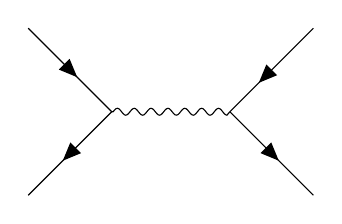
\begin{tikzpicture}
  \begin{feynman}
    \vertex (a) ;
    \vertex [below left=of a] (f2);
    \vertex [above left=of a] (f1);
    \vertex [right=of a] (b);
    \vertex [above right=of b] (f3) ;
    \vertex [below right=of b] (f4) ;

    \diagram* {
      (f1) -- [fermion] (a) -- [fermion] (f2),
      (a) -- [photon] (b),
      (b) -- [anti fermion] (f3),
      (b) -- [fermion] (f4),
    };
  \end{feynman}
\end{tikzpicture}
\caption{Feynman diagram}\label{PE}
\end{figure}
For example, the tildes line in figure \ref{PE} is the propagator of a virtue photon.

The most important propagator is \tbf{Feynman propagator}:
\begin{definition}[Feynman propagator]
  \begin{equation*}
    D_{F}(x-y)=\int \frac{\id^4p}{(2\pi)^4}\frac{i}{p^2-m^2+i\epsilon}e^{-ip\cdot(x-y)}
  \end{equation*}
\end{definition}
Feynman propagator can be written in terms of the Wightman function,
\begin{align}
  D_{F}(x-y)&=\int \frac{\id^4p}{(2\pi)^4}\frac{i}{p^2-m^2+i\epsilon}e^{-ip\cdot(x-y)}\\
&=\int \frac{\id^4p}{(2\pi)^4}\frac{i}{(p^0+E_p-i\epsilon)(p^0-E_p+i\epsilon)}e^{-ip\cdot(x-y)}\\
&=\int\frac{\id^3p}{(2\pi)^3}\frac{1}{E_p}e^{-ip\cdot(x-y)}\theta(x^0-y^0)+\int\frac{\id^3p}{(2\pi)^3}\frac{1}{E_p}e^{-ip\cdot(y-x)}\theta(y^0-x^0)\\
&=D(x-y)\theta(x^0-y^0)+D(y-x)\theta(y^0-x^0)\\
&=\expval{T\phi(x)\phi(y)}{0}\footnotemark
\end{align}
\footnotetext{\(T\) is the time ordering operator that indicates the operator in late time located on the left side.}
Feynman propagator will be used frequently in the real calculation, it corresponds to amplitude for free particle propagation.


















\newpage
\section{Quantum Electrodynamics}

%\section{Renormalization}

\newpage
\appendix
\addcontentsline{toc}{section}{Appendix~}

\section{Classical Field Theory}
\subfile{Appendix/Classical_Field_Theory}


\newpage





\end{document}